\documentclass[a4paper, 12pt]{article}

\usepackage[left=2cm, right=2cm, top=2cm]{geometry}
\usepackage{color}
\usepackage{graphicx}
\usepackage{float}

\begin{document}
\pagenumbering{roman}
\title{
		\textbf{Student Name:} Tevin Achong\\
		\textbf{Student ID:} 816000026\\
		\textbf{Course Code:} INFO3606\\
		\textbf{Course Title:} Cloud Computing\\
		\textbf{Assignment:} 2
		\date{March 10, 2020}
}
\maketitle

\newpage
\pagenumbering{arabic}

\begin{center}
	\textbf{Question 1}
\end{center}

\textbf{Limitations of leaf spine architecture:}
\begin{itemize}
\item
A large amount of cables and network equipment is required to scale the bandwith since each leaf must be connected to every spine device.
\begin{itemize}
\item
This can lead to more expensive spine switches with high port counts.
\end{itemize}
\item
The number of hosts that can be supported can be limited due to spine port counts restricting the number of leaf switch connections.
\end{itemize}

\textbf{Why we need Software-Defined Networking:}
\begin{itemize}
\item
\textit{Low-Cost Network Devices}:
\begin{itemize}
\item
Since intelligence is removed from devices in SDN it is not necessary to use costly network devices in the infrastructure layer.
\item
SDN promotes using low-cost network switches.
\item
An SDN controller manages the network using higher level policies as defined by applications.
\item
It performs all the control logic and gives instructions to network devices, which forward the packets or perform actions in accordance with instructions from the controller.
\end{itemize}

\item
\textit{Separation of Control Plane from Data Plane}:
\begin{itemize}
\item
The actions of the forwarding plane depend on different tables and logic such as whether to forward the incoming packet, drop the packet, or replicate the packet.
\item
The logic and algorithm underlying the actions of the forwarding plane need global knowledge of the network.
\item
Actions in a conventional network model are performed in the individual control planes of devices and the state of each and every device remains synchronized so that the entire network can continue working. 
\item
But with the introduction of network virtualization and multi-tenancy, several virtual devices need to be configured according to the requirements of the application.
\item
Hence SDN totally deactivates the control planes of individual devices and replaces them with a centralized controller that manages all forwarding planes.
\item
The first task of SDN is to separate the control plane of individual devices.
\end{itemize}

\item
\textit{Network Abstraction and Automation}:
\begin{itemize}
\item
SDN aims to provide network operators with a global view by hiding the internal workings of the network. SDN provides complete abstraction, so much so that the network programmer can easily obtain a global view without being aware of hardware-specific details.
\item
He can program the network requirements of applications simply by using NBI interfaces. 
\item
Network programmers no longer need concern themselves with individual device configuration, physical vendor-specific hardware details, or proprietary interfaces.
\end{itemize}

\item
\textit{Openness}:
\begin{itemize}
\item
SDN emphasizes open and standard protocols for communication between the controller and network devices (SBI) and communication between applications and the controller (NBI).
\item
Open interfaces allow interoperability among devices manufactured by different vendors. Open interfaces will also reduce the cost of networking devices.
\end{itemize}
\end{itemize}

\newpage
\begin{center}
\textbf{Question 2}
\end{center}

Network Function Virtualization (NFV), like SDN, is a network-related technique, the primary objective of which is to virtualize network functions such as load balancing, implementing firewall policies and routing, WAN optimization, and deep packet inspection. Back in the day, these functions were implemented using specialized expensive hardware. With the advent of NFV these functions are now implemented in software; this reduces the costs involved in setting up the network infrastructure of large enterprises. Because these functions are implemented using virtual machines and commodity hardware the network provisioning is simplified. NFV plays a crucial role in simplifying network management and provision in the transport, session, presentation, and application layers. The European Telecommunications Standards Institute (ETSI) defined the architecture of NFV and broke it down into three components: NFV infrastructure, virtualized network functions (VNFs), NFV management and orchestration (NFV MANO). Further, NFV helps operations support systems (OSS) to provide internal network requirements and business support systems (BSS) to deal with end users.\\
\indent
The NFV infrastructure comprises physical hardware made up of computing servers, storage devices, and network devices that are distributed across different geographical locations. This physical infrastructure is virtualized into a single logical virtual resource with the help of a virtualization layer on which different virtualized network functions are deployed.\\
\indent
Different networking functions that back in the day were implemented using specialized hardware - such as routers, firewalls, load balancers, switches, access control mechanisms, network address translation (NAT), content delivery network (CDN), and radio access network (RAN) - are now implemented using software, virtual machines (VMs), and commodity hardware. The virtualized network function elements are deployed on top of the NFV infrastructure.\\
\indent
NFV management and orchestration consists of three components: NFV orchestrator, virtualized infrastructure manager, and VNF manager; MANO provides orchestration and; life cycle management for virtualized software resources and other virtualization-related management tasks.

\begin{figure}[H]
	\centering
	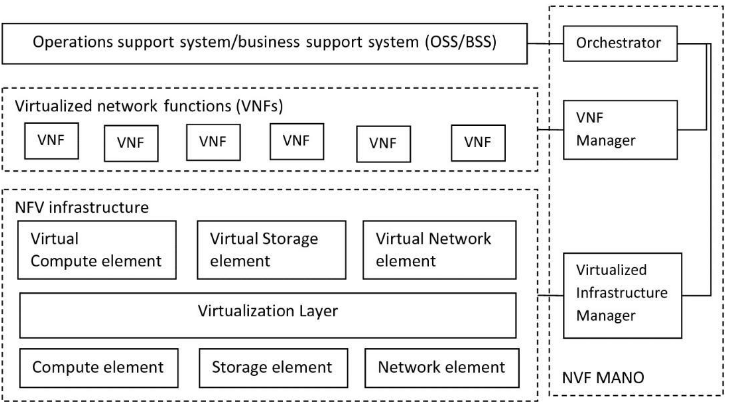
\includegraphics[width=\linewidth]{nfv.png}
  	\caption{Architecture of NFV}
	\label{fig:nfv}
\end{figure}


\newpage
\begin{center}
\textbf{Question 3}
\end{center}

\begin{itemize}
\item
Modern enterprise networks and data centers are large and span a number of buildings. 
\item
They employ virtualization to hide heterogeneity in hardware.
\item
This led inevitably to huge east-west traffic within enterprise networks.
\item
Traffic within large enterprises needs to be effectively handled with deterministic latency. 
\item
The number of servers and devices keep on increasing as do the number of virtual servers. 
\item
For example, around 20 virtual servers can be configured on a single physical server.
\item
Data centers typically contain around 100,000 physical servers.
\item
Hence a huge number of virtual servers are involved in data centers.
\item
To support multiple tenants data centers adopt network virtualization. 
\item
Each tenant has his/her own virtual network, which must be logically separated from other virtual networks.
\item
Everyday digitization of data drives tremendous changes in customer demands and hence enterprises have to evolve to satisfy a wide variety of use cases:
\begin{itemize}
\item
videoconferencing applications
\item
video sharing and video games
\item
video surveillance applications
\item
real-time processing of streaming data
\item
situational awareness applications with robotics
\item
big data applications
\item
IoT applications
\item
natural language applications
\end{itemize}
\item
Typically, most use cases either require
\begin{itemize}
\item
huge storage of data
\item
huge computing power to process data
\item
huge networking capabilities to send and receive data
\end{itemize}
\item
The need for business agility drives the automation of networking.
\item
For example, after testing a code in the development environment let us consider the code is to be moved to the integration and production environments.
\item
When software is moved to different environments, configuring the required security policies, access policies, and routing policies in each environment becomes essential.
\item
In addition, the movement of software among different environments will happen on a daily or weekly basis in an Agile enterprise. 
\item
In such a scenario manual configuration of the policies required in each environment will become impractical. 
\item
This drives the automation of networking configuration.
\item
Network performance includes such features as high bandwith, low latency, low jitter, and no packet loss.
\item
On the one hand, external customers expect very low latency when they interact with enterprise websites.
\item
On the other hand, such business processes as manufacturing and monitoring require very frequent data exchange with very low latency.
\item
Hence it is essential to include various enterprise networking solutions such as
\begin{itemize}
\item
WAN optimization
\item
static routes
\item
migration of servers to nearest points, and
\item
caching contents
\end{itemize}
\item
As the enterprise network spans across different locations, visibility and control of network devices has to be met with a global view of devices.
\item
It is up to enterprises to ensure that services are offered in line with agreed services levels (as per the SLA) and have sufficient path redundancy.
\item
Suitable load balancing has to be ensured for peak loads.
\item
Security is brought about by making use of a number of security mechanisms such as
\begin{itemize}
\item
authentication and identity management
\item
access control
\item
firewalling
\item
single sign-on
\item
data loss prevention
\item
fraud detection
\item
malware detection
\item
intrusion detection and prevention
\item
audit records
\end{itemize}
\item
Security is an important concern as enterprise networks span multiple domains and different service provider sites.
\item
These requirements make it clear that enterprise networking has to offer quality of service not only in bandwith or performance but in many other areas as well.
\item
Enterprise networks cannot stand alone from computing or storage technologies.
\item
Networking techniques should grow in line with the speed of computing and storage because the use cases of business processes are becoming increasingly agile and dynamic.
\item
The digitization of data drives three major tasks:
\begin{itemize}
\item
data storage
\item
data transformation
\item
data transfer
\end{itemize}
\item
All three tasks essentially need networking capabilities.
\item
Ensuring networking capabilities are optimized is essential when data and processes are not in same location.
\item
Since data gets distributed the processing of data is done in a distributed manner along with parallel processing techniques.
\item
This is essentially responsible for bringing a very large amount of internal traffic to the enterprise network.
\item
Hence large enterprises and data centers prefer another network architecture called leaf spine architecture.
\item
In leaf spine architecture servers are connected to leaf switches
\item
Each leaf is connected to every spine
\item
There is no direct spine-to-spine or leaf-to-leaf connection in this architecture
\item
The leaf layer consists of access switches that connect to devices such as servers.
\item
The spine layer is the backbone of the network and is responsible for interconnecting all leaf switches.
\item
The path is randomly chosen so that traffic load is evenly distributed among the switches of the spine layer.
\item
The ease of expansion optimizes the IT department's process of scaling the network. 
\item
The important aspect of this architecture is that every server can reach every other server with the same number of hops.
\item
This makes network latency predictable and consistent.
\item
In this architecture the spine layer is the backbone of the network and is responsible for interconnecting all leaf switches.
\item
As enterprises move from on-premises enterprise infrastructures to the cloud infrastructure there is a need not only to consider the architecture of applications but also network architecture models.
\item
Traditionally, enterprises provided the typical tiers of an application - client tier, business logic tier, and database tier - in different servers and interconnected those servers by means of the network infrastructure.
\item
In the 2010s enterprises adopted the service-oriented architecture (SOA) model to develop business applications and achieve business agility.
\item
One of the tenets of this development was to promote reusability and interoperability.
\item
SOA provides application-to-application interactions with the help of an enterprise service bus (ESB).
\item
An ESB serves as the central location to integrate applications using a loosely coupled, asynchronous, reliable, and secure messaging model.
\item
Although an ESB provides centralized integration of applications, it is inflexible.
\item
An ESB is basically used to integrate different applications, whereas recent microservices architecture (MSA) provides the architecture to develop applications in the form of microservices.
\item
Microservices are autonomous, self-contained, and self-deployable. This makes deployment much easier.
\item
Whenever there is a change in a service, only that particular service is redeployed.
\item
In contrast to a traditional monolithic or SOA-based application, which treats all functions as a single process, MSA treats each service as a process. 
\item
These services can communicate with one another using HTTP.
\item
Moreover, a microservice can be manipulated through its application programming interface (API).
\item
In much the same way as they have modernized their application architecture, enterprises primarily focus on the recent software development process model - namely, Agile - in contrast to the old waterfall or other models.
\item
They do so because the Agile model accepts changing and dynamic customer demands and emphasizes continuous integration and continuous delivery of software development.
\item
When an application is developed in a traditional manner, continuous delivery becomes difficult.
\end{itemize}
  

\newpage
\begin{center}
\textbf{Question 4}
\end{center}

NAS devices make use of the TCP/IP network for file sharing. During this file sharing, at a high level:
\begin{itemize}
\item
Clients mount the remote file system into their machines (a Windows client has to mount CIFS and a Unix client mounts NFS).
\item
Clients can view files, create files, retrieve files, change files, etc.
\end{itemize}

Internally:
\begin{itemize}
\item
When clients make a request to retrieve a file they use an NFS or CIFS request.
\item
Clients submit a high-level file I/O request to the NAS gateway.
\item
The NAS gateway converts the high-level file I/O request into a block-level request with details of the actual blocks where the file is stored, can be written to, or retrieved from the disk.
\item
The disk produces a block-level I/O response.
\item
The NAS gateway again converts the block-level I/O response into a file-level I/O response and returns it to the client. It is the NAS gateway that performs all the internal operations and allows very simple file-sharing access to the clients in a network.
\end{itemize}

\textbf{Since NAS devices make use of the TCP/IP network for file sharing, a considerable amount of the bandwith available will be utilized by NAS devices.\\ 
NAS is less efficient since data transfer is on top of the TCP/IP}.

\newpage
\begin{center}
\textbf{Question 5}
\end{center}
From the description of the case study, we know that each of the company's branches has its own dedicated FC SAN; so we know that they have access to the high performance and high scalability provided by FC SAN. However, these advantages of FC SAN bring with them the burden of the additional cost of buying FC components such as HBA, FC switches, and establishing the FC fabric. \textbf{One solution Gamma can use to interconnect their storage networks at low cost with no distance limitation is to use Internet Protocol Storage Area Network (IP SAN), using the internet Small Computer System Interface (iSCSI).}\\
\indent
IP SAN is a type of Storage Area Network that has the aim of transporting storage traffic over the existing TCP/IP network using protocols like internet SCSI (iSCSI). Since, from the specification of the case study, we know that the different locations are connected through TCP/IP, using IP SAN is a definite possibility.\\

The architecture of IP SAN is as follows:

\begin{figure}[H]
	\centering
	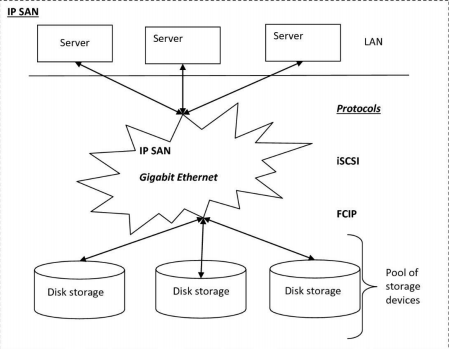
\includegraphics[width=\linewidth]{ip_san_architecture.png}
  	\caption{The architecture of IP SAN}
	\label{fig:ip_san_architecture}
\end{figure}

\begin{itemize}
\item
The internet is the primary medium and backbone used to share massive amounts of all kinds of digital information, such as text, audio, and video, in a highly distributed way.
\item
The growing trend of digitization requires a huge amount of network storage space. 
\item
Each of the protocols in the TCP/IP network are used for communication.
\item
The primary advantage of IP SAN is that networked storage can be made available at any place wherever there is a TCP/IP network.
\item
Another advantage is that there is no need to procure special hardware since the network is already existing.
\item
Hence the cost involved in IP SAN is very low.
\end{itemize}

\textit{\underline{Internet Small Computer System Interface (ISCSI)}}
\begin{itemize}
\item
\textbf{iSCSI is the most common protocol used in IP SAN.}
\item
Small Computer System Interface (SCSI) is one of the standard interfaces and command sets used to transfer data between computers and disk storage, whereas internet SCSI (iSCSI) uses the same SCSI command set to communicate between computing devices and storage devices via a TCP/IP network.
\item
iSCSI is a storage networking protocol stack that allows storage resources to be shared over an IP network. iSCSI is a mapping of the SCSI protocol over TCP/IP.

\begin{figure}[H]
	\centering
	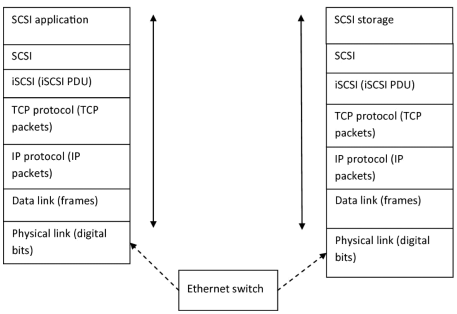
\includegraphics[width=\linewidth]{iscsi_tcpip.png}
  	\caption{iSCSI over the TCP/IP storage network}
	\label{fig:iscsi_tcpip}
\end{figure}

\item
Using SCSI initiates and SCSI request that is mapped onto the internet by the iSCSI layer.
\item
At they physical layer, iSCSI supports a Gigabit Ethernet interface that enables systems supporting iSCSI interfaces to be directly connected to standard Gigabit switches and IP routers.
\item
The iSCSI protocol sits above the physical and data link layers and interfaces to the operating system's standard SCSI access method command set. IP SAN uses TCP as a transport mechanism for storage over Ethernet and iSCSI encapsulates SCSI commands into TCP packets, thus enabling the transport of I/O block data over IP networks.

\begin{figure}[H]
	\centering
	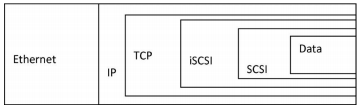
\includegraphics[width=\linewidth]{scsi_encap.png}
  	\caption{Encapsulation of SCSI commands into TCP/IP}
	\label{fig:scsi_encap}
\end{figure}

\item
iSCSI can be supported over all physical media that support TCP/IP as a transport, but today's iSCSI implementations are on Gigabit Ethernet.
\item
The iSCSI protocol runs on host initiator and on the receiving target device. iSCSI can run in software over a standard Gigabit Ethernet network interface card (NIC) or can be optimized in hardware on an iSCSI host bus adapter (HBA) for better performance.

\begin{figure}[H]
	\centering
	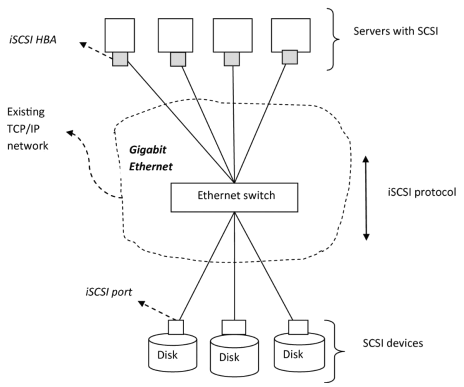
\includegraphics[width=\linewidth]{ipsan_iscsi.png}
  	\caption{Implementation of IP SAN and iSCSI}
	\label{fig:ipsan_iscsi}
\end{figure}

\item
There are three key components for iSCSI communication in IP SAN:
\begin{itemize}
\item
iSCSI initiators
\item
iSCSI targets
\item
An IP-based network
\end{itemize}
\item
An iSCSI initiator sends commands and associated data to a target and the target returns data and responses to the initiator.
\item
IP SAN using iSCSI is composed of initiators and targets connected by an IP network in which the server acts as the initiator or iSCSI host and the iSCSI storage device acts as the target. iSCSI storage devices and iSCSI servers are connected using one of the following four types of iSCSI interface:
\begin{itemize}
\item
a standard NIC with a software iSCSI adapter
\item
a TCP offload engine (TOE) NIC with a software iSCSI adapter
\item
an iSCSI HBA
\item
a converged network adapter (CNA)
\end{itemize}
\end{itemize}


\textit{\underline{Justification of the use IP SAN:}}
\begin{itemize}
\item
IP SAN does not require a separate network to manage connections to storage systems. It uses the existing TCP/IP network to create the storage area network. Hence the cost of creating an IP SAN is much less than is the case with other networks.\item
\textbf{IP SAN does not have any distance limitation.} Hence an enterprise can establish its data center at any location where its network is over a LAN, WAN, or the internet. This allows IP SAN to be used flexibly and conveniently at any place to establish disaster recovery.
\item
IP SAN can co-exist with FC SAN. Hence an enterprise has the option of combining IP SAN with an already existing FC SAN to keep investment costs for storage to a minimum. Since each branch of Gamma has its own dedicated FC SAN, this is ideal for them.
\item
IP SAN can use either a specialized HBA to connect servers to the SAN or just use standard NIC cards/Ethernet ports to do the same. This enables server I/O consolidation and reduces complexity/cost.
\item
Gigabit Server Adapters (NIC cards) can be used to connect to the network and thereby provide the Gigabit speeds so necessary today.
\item
Implementation and maintenance of IP SAN is easier than is the case with other networks.
\item
IP SAN is highly suitable when implementing a SAN in virtual server environments.
\end{itemize}



\newpage
\begin{center}
\textbf{Question 6}
\end{center}

There are three standard data access methods:
\begin{enumerate}
\item
File-level access
\item
Block-level access
\item
Object-level access
\end{enumerate}

\begin{itemize}
\item
\textit{File-Level Access}

\begin{itemize}
\item
In file-level access the file system is created on a separate file server at the storage device end and the file-level request is sent over a network.
\item
Because data are accessed at the file level this method has a higher overhead than data accessed at the block level.
\item
File-based storage is usually accessed via a standard protocol like NFS or SMB/CIFS.
\item
Fixed file attributes, such as type, size, date created, and date modified, are stored in the file system. 
\item
File-based storage is good for sharing files and sharing directories over a LAN or WAN.
\end{itemize}

\item
\textit{Block-Level Access}
\begin{itemize}
\item
In block-level access, the file system is created on a client compute system, and data are accessed on a network at the block level.
\item
In this case raw disks or logical volumes are assigned to the compute system, which the client compute system can format to create its own file system.
\item
Access to block storage is usually through a client on the operating system over the FC.
\item
Block storage is ideal for databases or VMs.
\item
The block-level access mechanism is the typical data access mechanism used in SAN.
\item
Data access in this mechanism is done in terms of blocks of fixed size.
\item
The tpyical block size in most scenarios is 512 bytes.
\end{itemize}

\item
\textit{Object-Level Access}
\begin{itemize}
\item
In object-level access data are accessed in terms of variable-sized chunks called objects.
\item
Each object gets a unique identifier called an object identifier (OID), which is calculated from the file content and the metadata.
\item
Applications access the object using this OID. The OID is generated with the help of a 128-bit random number generator, which helps to ensure that the OID is unique. Other details about the object, such as location and size, are stored in the form of metadata. Data that are stored in object-based storage devices can be accessed using web service APIs such as Representational State Transfer (REST) and Simple Object Access Protocol (SOAP). Some types of object-based storage devices also offer support for protocols such as Hyper Text Transfer Protocol (HTTP) and XML.
\end{itemize}
\end{itemize}

\textbf{Advantages of Object-Level Data Access:}
\begin{itemize}
\item
Object-based storage devices incur much less overhead when performing concurrent read/writes, file locks, and permissions.
\item
This significantly improves performance and gives massive scaling capabilities to object-based storage devices.
\item
In addition, the amount of rich metadata associated with each object helps in carrying out analytical operations very efficiently.
\item
Hence object-based storage devices are ideal candidates for storing data that are generated/used by high-performance big data applications.
\end{itemize}

\newpage
\begin{center}
\textbf{Question 7}
\end{center}

\textbf{The point of software-defined storage:}

\begin{itemize}
\item
The goal of software-defined storage is to provide administrators with flexible management capabilities through programming.
\item
A single software interface can be used to manage a shared storage pool that runs on commodity hardware.
\item
Whether storage is virtualized or not, SDS provides a simple managing interface that automates the tasks of managing storage.
\item
SDS is a management API that provides a standard way of configuring software devices.
\item
This API hides the heterogeneity in devices, vendors, hardware, etc.
\item
This makes it easier for database administrators to configure devices automatically through software.
\item
There is no need to set the required parameters in hardware, and by so doing human error during configuration is prevented.

\begin{figure}[H]
	\centering
	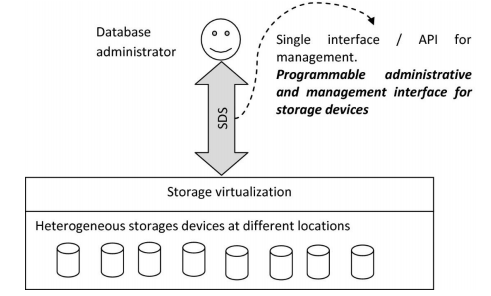
\includegraphics[width=\linewidth]{sds.png}
  	\caption{Concept of software-defined storage}
	\label{fig:sds}
\end{figure}
\end{itemize}

\textbf{Key characteristics of Software-Defined Storage:}
\begin{itemize}
\item
Abstraction: In SDS architecture the software that manages storage decouples and abstracts the heterogeneity in hardware, vendors, etc.
\item
Automation: In SDS the configuration and management tasks of storage devices are automated using software configurations, scripts, etc.
\item
Industry standards: SDS solutions rely on industry standards and hence prevent vendor lock-in.
\item
Scalability: SDS supports the concepts of virtualization and hence SDS makes it easier to add or remove storage devices.
\item
Flexibility: SDS allows users to choose hardware according to their needs and removes the constraint of  having to deal with a specific vendor.
\item
Virtualization: SDS architecture pools together storage resources and manages them as a cohesive unit. It virtualizes storage devices in much the same way as server or network virtualization.
\end{itemize}

\textbf{Running in a Docker container is an example of a Container-based software-defined storage that exists in the market today.}
\end{document}